\section{Paralelní vkládání (Paralel Insertion)}
\subsection{Provedení nad automatem}
Provedení paralelního vkládání je velice podobné vkládání sekvenčnímu, nejednodušší bude opět si uvést příklad. Mějme tedy opět dva jazyky $K(M)=\{CD\}$ a $L(N)=\{AA, BB\}$ a automaty kterými jsou definovány, viz výše uvedený příklad pro sekvenční vkládání(\ref{imgExample:insertionTeory});

Rozdíl je zde v tom, že při paralelním vkládání, musíme vždy po zpracování znaku z řetězce jazyka $K(M)$, zpracovat celý řetězec z jazyka $L(N)$. Abychom použili analogii na na osy $X$ a $Y$, tak vždy když se chceme posunout po ose $X$, musíme se posunout po ose $Y$ až do konečného stavu. (viz \ref{imgExample:paralelinsertionResult})
\begin{figure}[H]
\centering
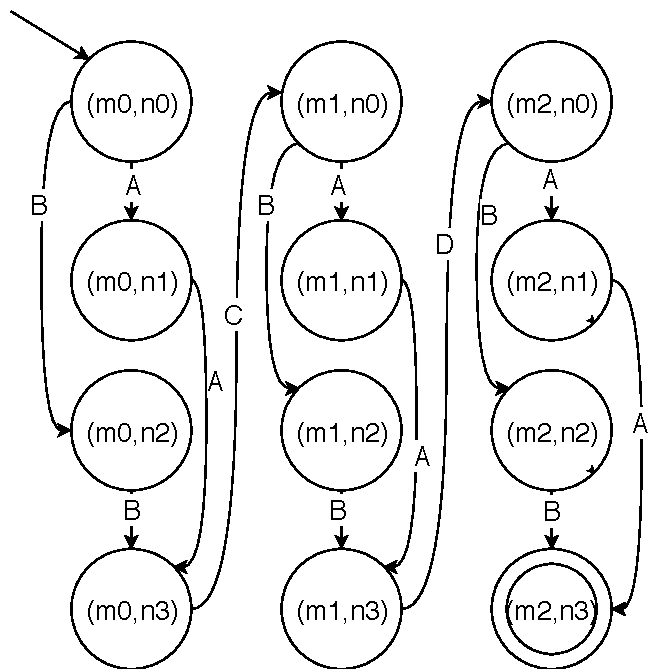
\includegraphics[width=0.7\textwidth]{obrazky-figures/paralelInserionResult.pdf}
\label{imgExample:paralelinsertionResult}
\caption{Automat generovaný operací ParalelInsertion(N,L)}
\end{figure}

Tento příklad si můžeme zobecnit následujícím způsobem, mějme dva automaty :
$M=\{Q_{M}, \Sigma_{M}, \delta_{M},s_{M}, F_{M}\}$ a $N=\{Q_{N}, \Sigma_{N}, \delta_{N},s_{N}, F_{N}\} $

Paralelní vkládání poté můžeme zobecnit následovně:
\begin{equation}
\label{eqA:ParalelInsertion}
\begin{split}
    ParalelInsertion(M,N) = \{ &\\
           &Q = Q_{M} \times Q_{N},\\
    &  \Sigma = \Sigma_{M} \cup \Sigma_{N} \\
    & \delta = \{ (q_{M},q_{N})\alpha \longrightarrow \left\{\begin{matrix}
 (q_{M}\alpha, s_{N})& if & q_N \in F_{N}\\ 
 (q_{M}, q_{N}\alpha)& else & 
\end{matrix}\right.;\\
    &\tab q_{M} \in Q_{M} \land q_{N} \in Q_{N} \land \alpha \in \Sigma\\
    &\tab\}, \\
    & s = (s_{M}, s_{N}), \\
    & F = F_{M} \times F_{N} \\
    \}&
\end{split}
\end{equation}



\subsection{Implementace}
Pravidla se vytváří dle výše uvedeného automatu, obdobně jako tomu bylo v ukázce \ref{example:shuffle}
(\textit{src/operations/parallelInsertionFA.js})
% \begin{figure}[h]
% \centering
% \includegraphics[width=0.7\textwidth]{obrazky-figures/intersectionExample.png}
% \label{imgExample:intersection}
% \caption[]
%     {\tabular[t]{@{}l@{}}Ukázka implementace operace Intersection \\ $src/operations/intersectionFA.js$\endtabular}
% \end{figure}
